\begin{figure}[htbp]
    \begin{subfigure}{.5\textwidth}
    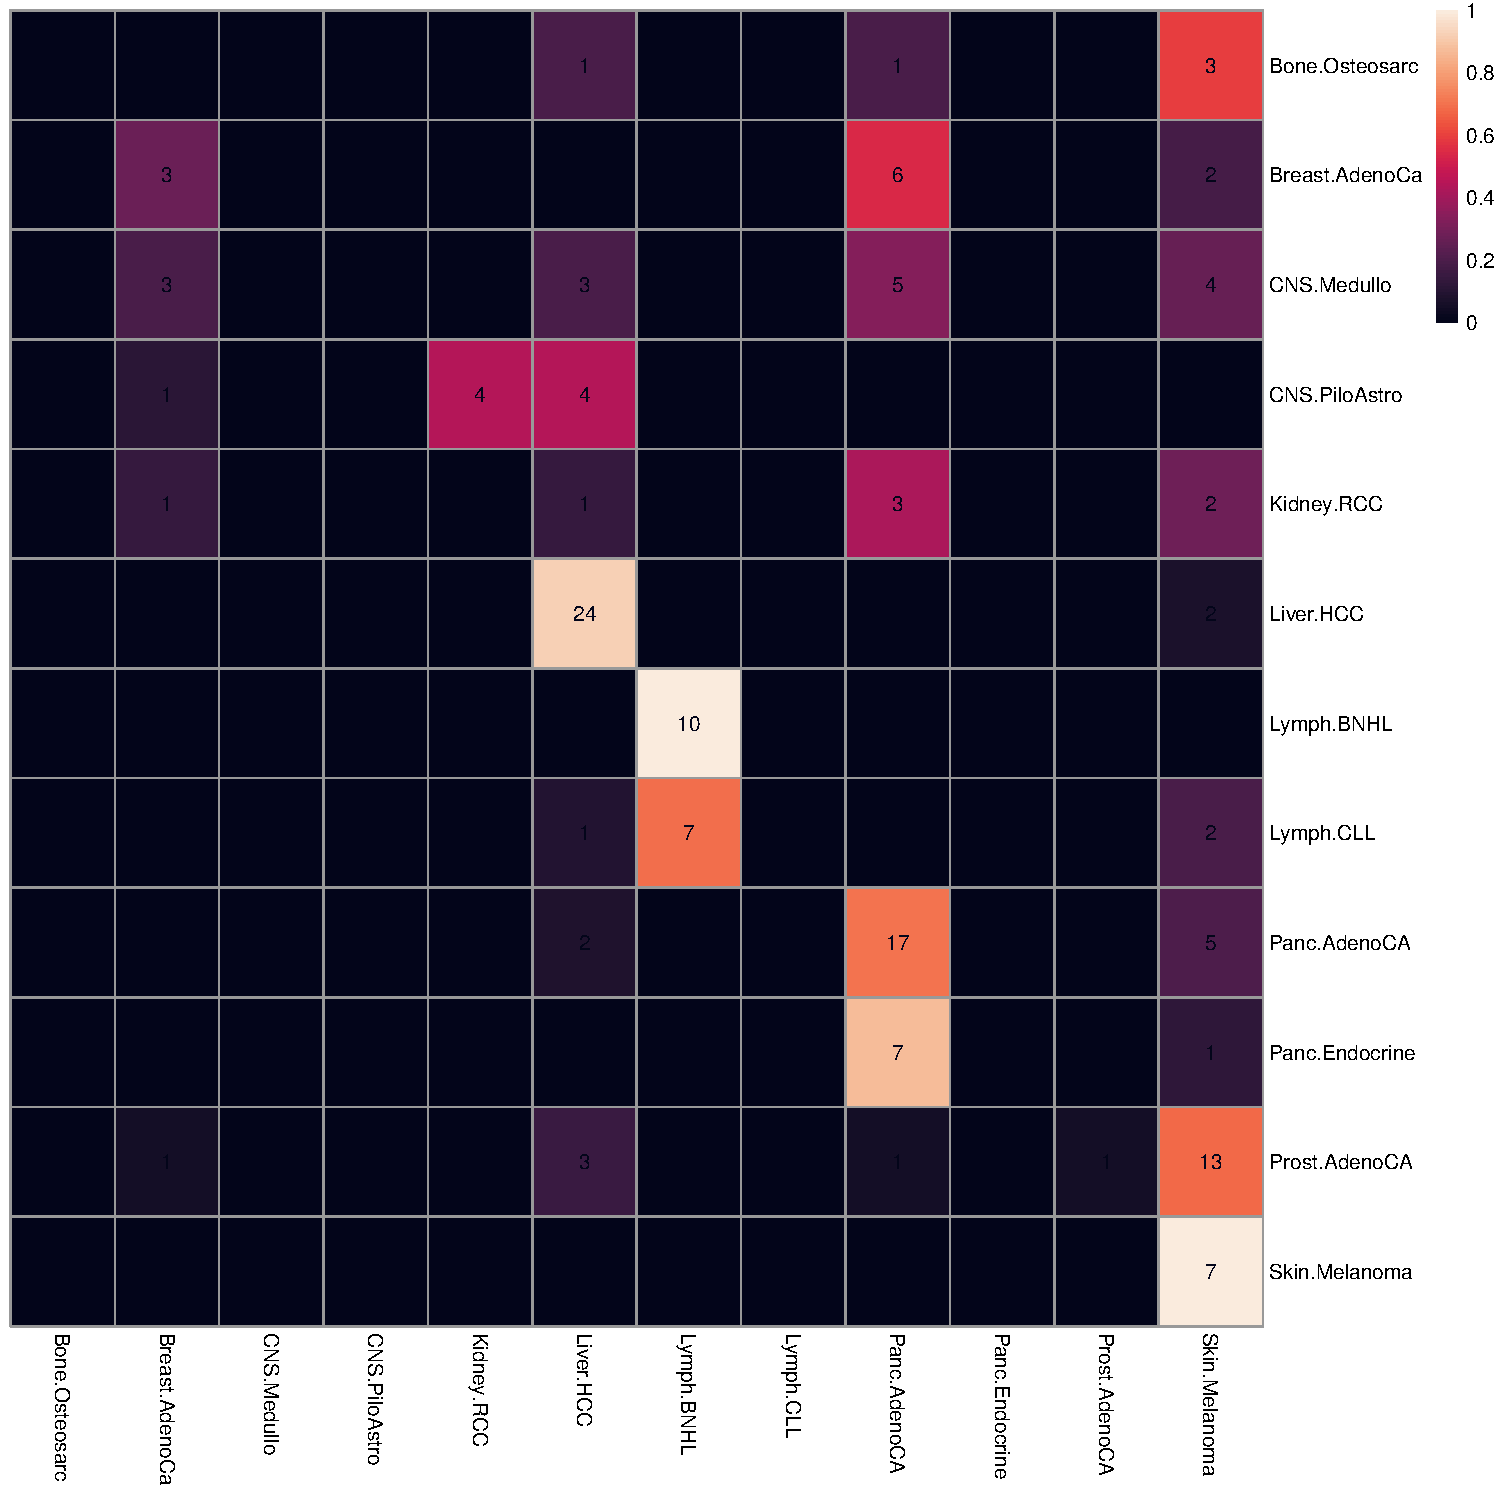
\includegraphics[scale=0.6]{graphics/confustion_matrix_bins_euclidean.pdf}
    \caption{Bins/Euclidean}
    \label{fig:bin_euclidean}
    \end{subfigure}
    ~
    \begin{subfigure}{.5\textwidth}
    
    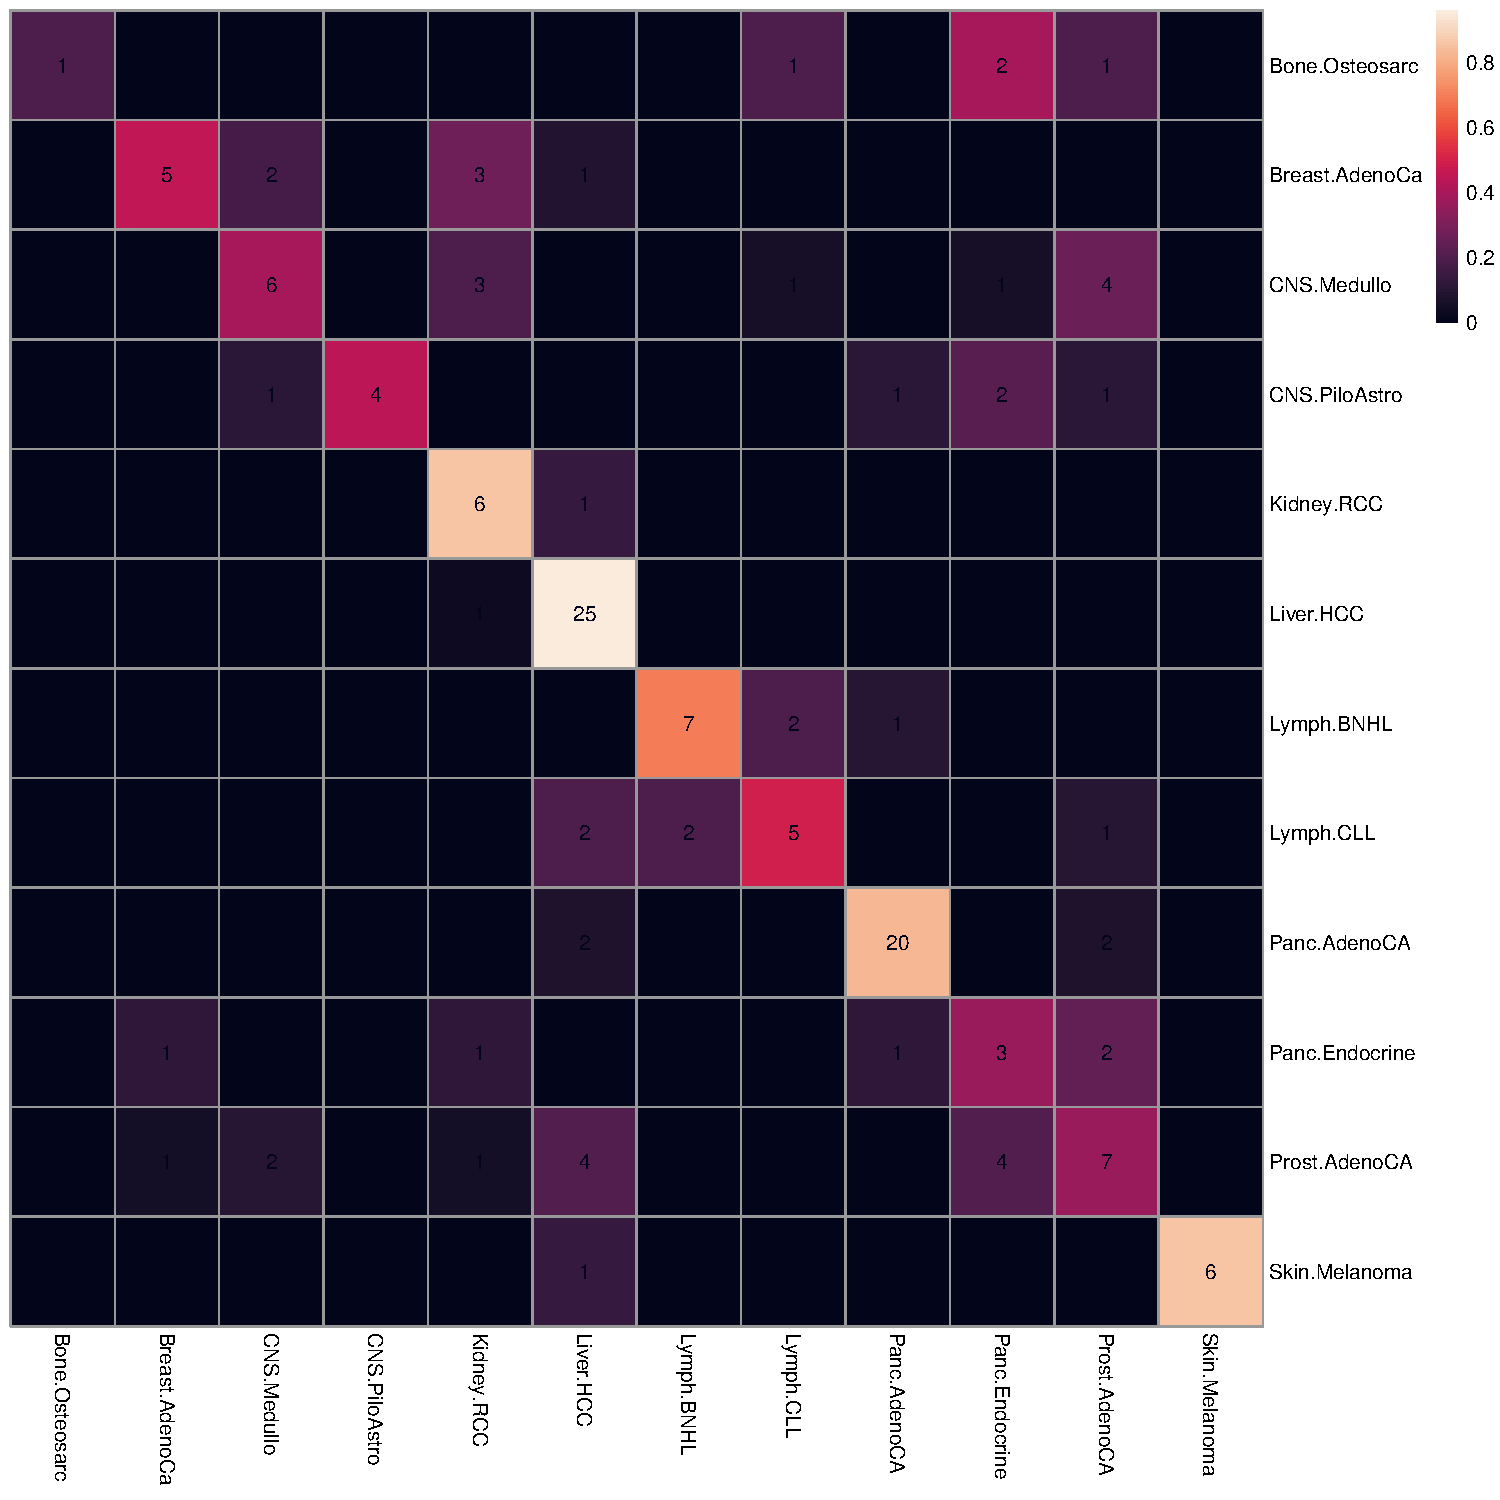
\includegraphics[scale=0.25]{graphics/confustion_matrix_smooth_euclid.pdf}
    \caption{Smooth/Euclidean}
    \label{fig:smooth_euclidean}
    \end{subfigure} \\
    \vspace{0.5cm}
    
    \begin{subfigure}{.7\textwidth}
    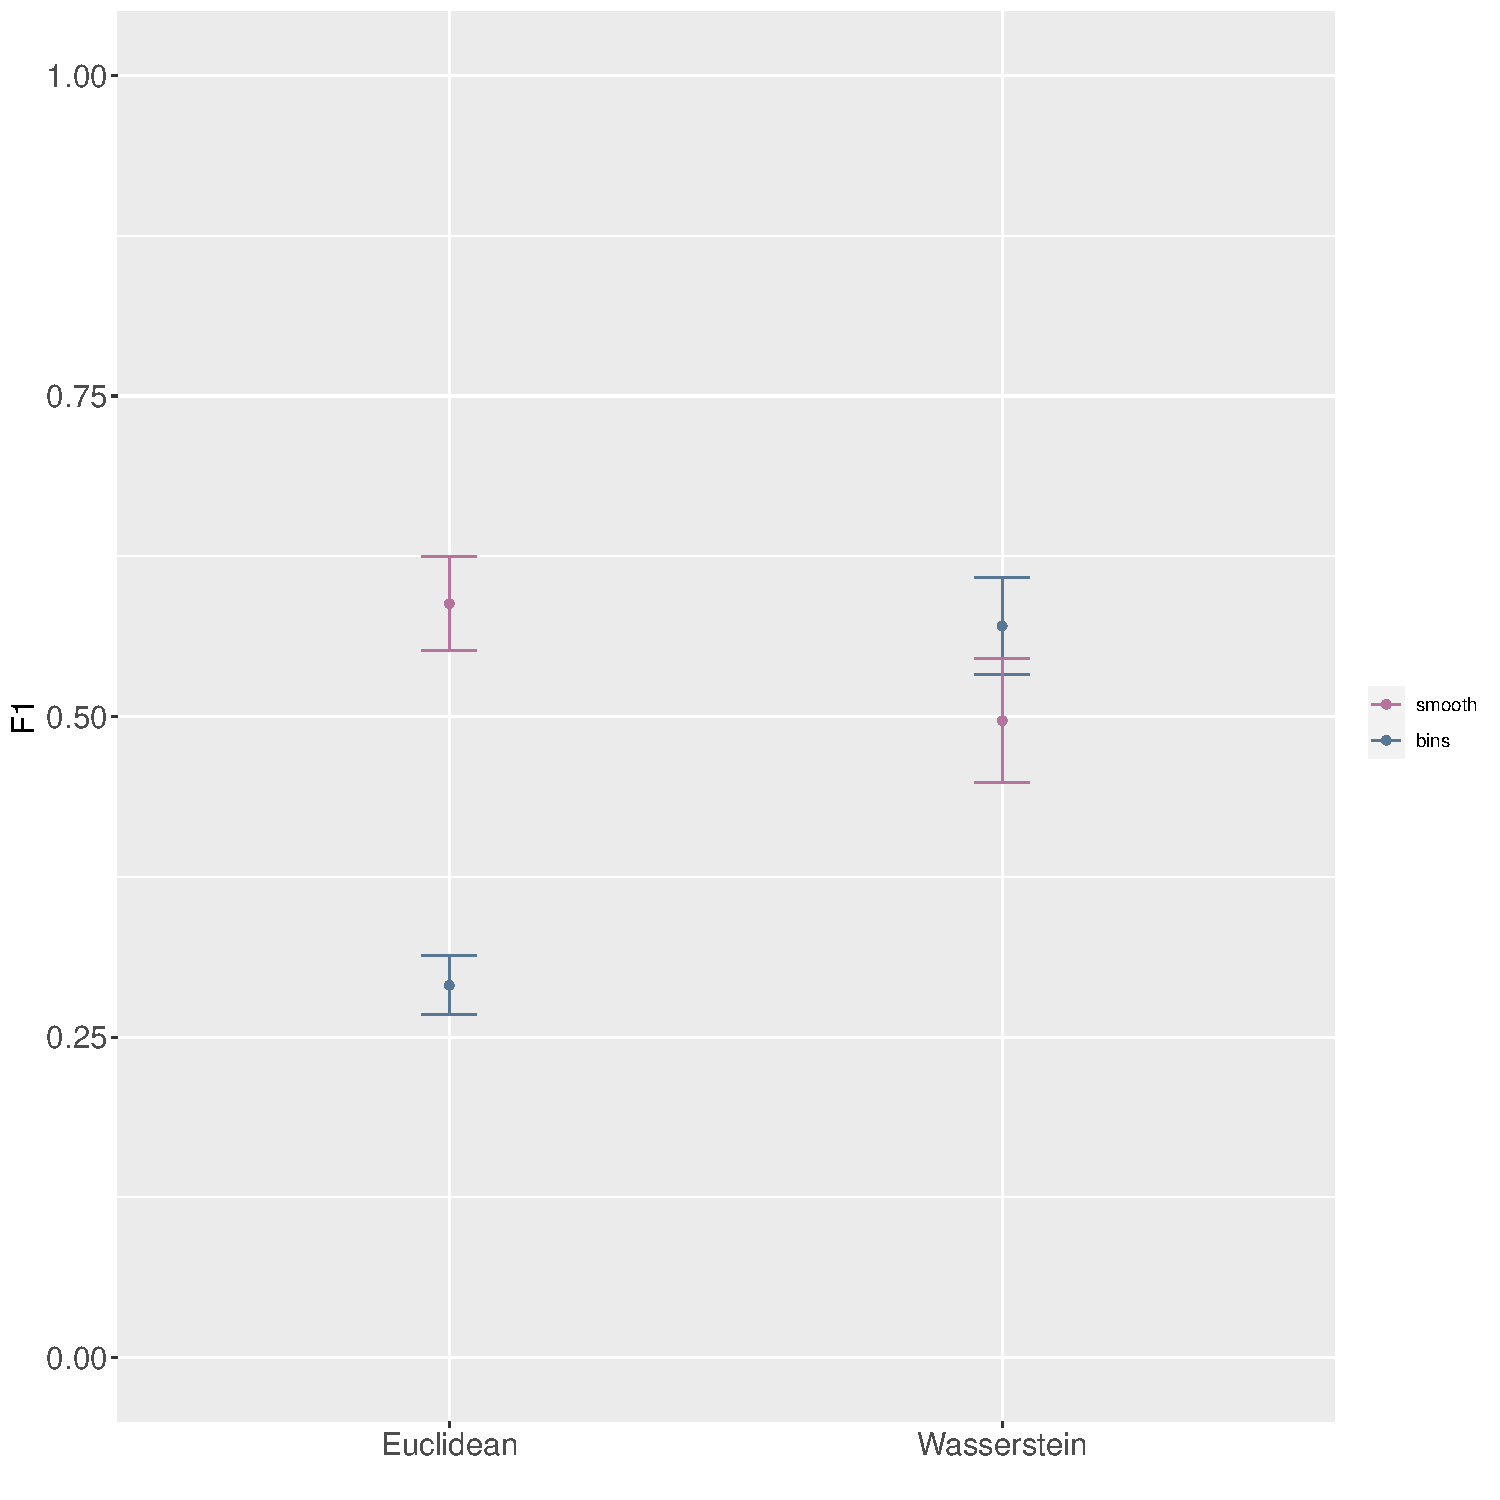
\includegraphics[scale=0.8]{graphics/f1_gle.pdf}
    \caption{F1 summary}
    \label{fig:f1_gle}
    \end{subfigure}
    
    
    \caption{\textbf{Base substitutions are a rich source of information, manifested by $RE$}. Here, $RE$'s are shown in sequence logos for (a) Skin-Melanoma (b) Kidney-RCC (c) Liver-HCC (d) Panc-AdenoCA. For each panel, each row was derived from a GLM. The x-axis is the wildtype base; the y-axis is the product of the substitution. The heights of the letters are $RE$'s. An up-orientation indicates an excess while a down-orientation indicates a deficit of the mutation.}
    \label{fig:ml_gle}
\end{figure}